\documentclass[11pt]{article}
\usepackage{array}
\usepackage{tabularx}
\usepackage{graphicx}
\usepackage{algorithm}
\usepackage{algorithmic}
\usepackage{pgfplotstable}
\usepackage{pgfplots}
\usepackage{filecontents}
\usepackage{amsmath}



\title{
	\textbf{IMS Assignment 4}
}

\author{Tobias Stahl \\ 10528199 \and Ioannis Giounous Aivalis \\ 10524851 }

\begin{document}

\maketitle

\section{Introduction}
This report is about Assignment 4 of the UvA course Intelligent Multimedia Systems. The goal of the first part of Assignment 4 is to implement functions to align images using the SIFT \footnote{http://
www.vlfeat.org/} implementation and implement a RANSAC algorithm.\\
The second part is about stitching two images together.

\section{Exercise 1}
In this part of the assignment six images of a boat from different angles are used to affine them to each other. Using the SIFT implementation the matching regions between two images are found.\\
Applying the RANSAC algorithm, the best transformation parameters are found. The process to do that is as follows:

\begin{itemize}
	\item 	Repeat N times
	\item	Randomly select three matches of all matches
	\item	Compute transformation matrix
	\item	Transform all regions in matches
	\item	Count inliers
	\item	If there are more inliers with this setting than with the previous best setting, keep the 			matrix
	\item	After all iterations are done, transform the image with the best transformation matrix
\end{itemize}

The subset of three regions out of the set of matches is chosen, since this is the minimal number of regions needed to solve an affine transformation.\\
We observed that we end up with good transformation parameters already after two iterations most of the time. To be sure we choose a setting of four iterations in the submitted \texttt{demo1.m}, since it rarely happens that the parameters are too bad after two iterations.\\
In order to transform the image, a function \texttt{transformImage.m} is implemented for one thing, for another thing the Matlab built-in functions \texttt{maketform\-('affine' )} and \texttt{imtransform()} are used.\\
Running \texttt{demo1.m} will affine each image of the boat to all other images and output and save the comparisons of the built-in function to our \texttt{transformImage()} function in a plot. With the boolean parameter \texttt{plotFig} it can be choosen, if the plot of the two images side-by-side with the connecting line of the corresponding points appears.\\
An example of the comparison of the two functions is shown in Figure ~\ref{affine}. Figure ~\ref{side_by_side} shows an example of the two images side-by-side.\\
The other images of the affined images are supplied in the submitted zip-file.

\begin{figure}[h!]
\begin{flushleft}
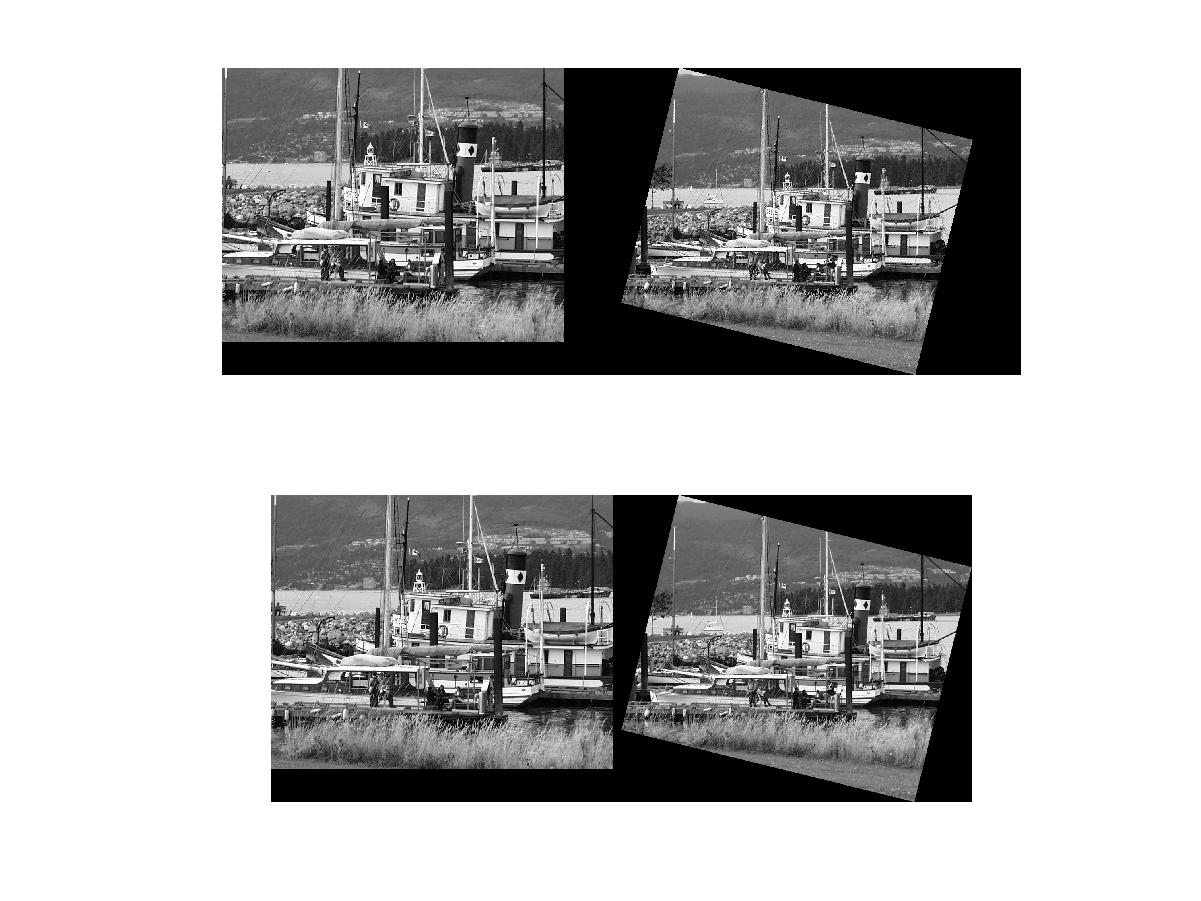
\includegraphics[scale=0.4]{Comparing1_2.jpg}
\caption{Comparing the affine functions for images one and two. The \texttt{transformImage()} function is on top, he Matlab built-in function is on the bottom.}
\label{affine}
\end{flushleft}
\end{figure}

\begin{figure}[h!]
\begin{flushleft}
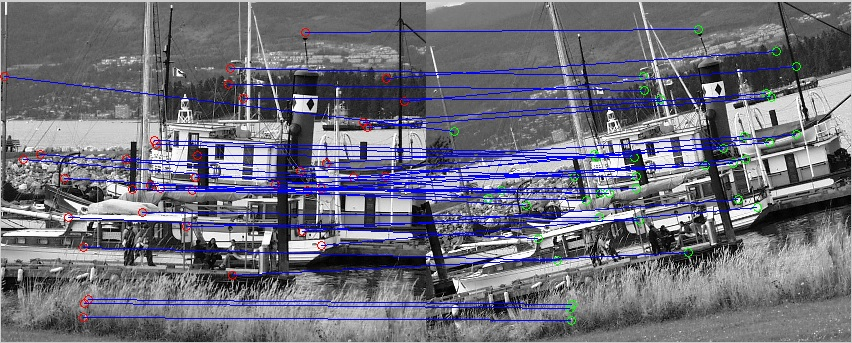
\includegraphics[scale=0.7]{side_by_side.jpg}
\caption{The two images side-by-side with a connecting line between their corresponding points.}
\label{side_by_side}
\end{flushleft}
\end{figure}

\subsection{Exercise 2}
In this exercise two images of a train from different angles are supposed to be stitched together using the previous mentioned algorithms. Figure ~\ref{stitched} shows the original images side-by-side with the resulting stitched image.

\begin{figure}[h!]
\begin{flushleft}
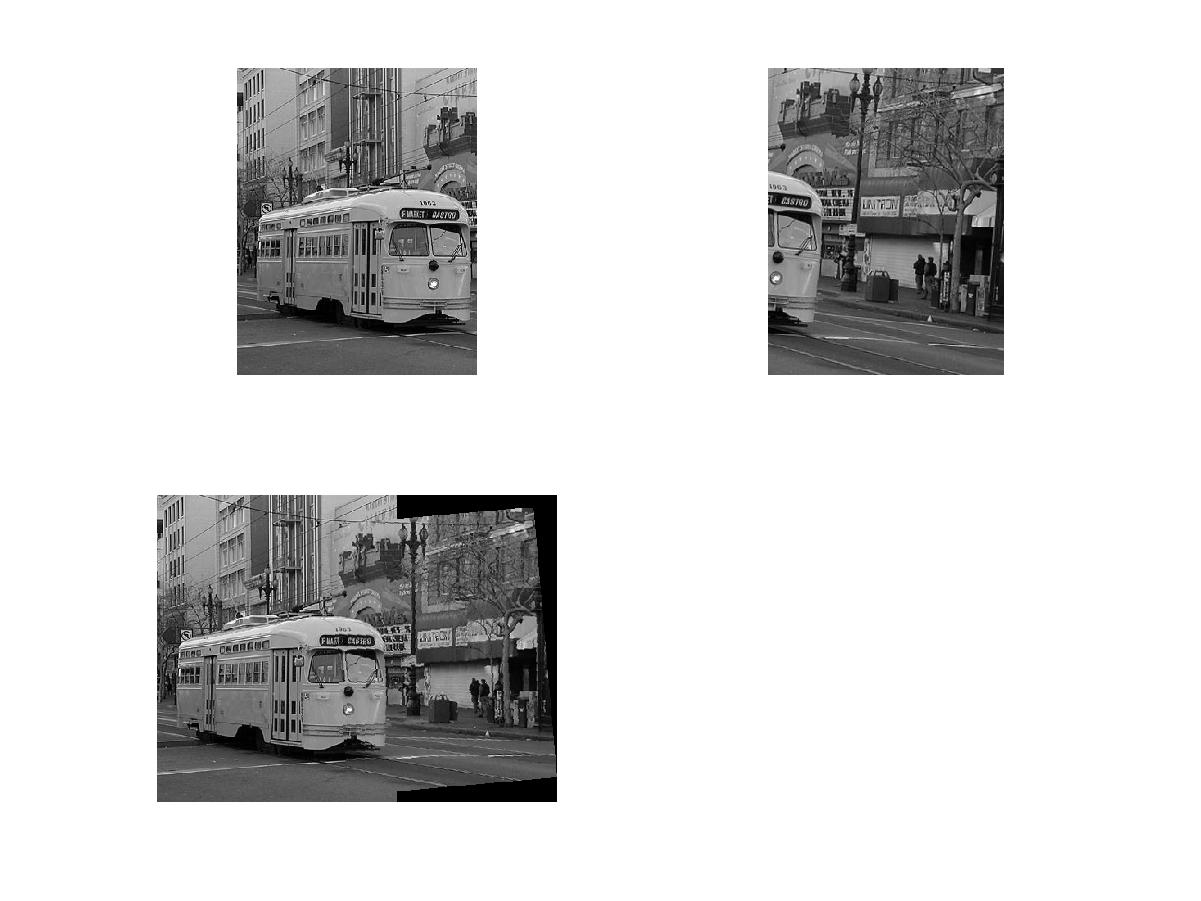
\includegraphics[scale=0.4]{stich.jpg}
\caption{The two original images side-by-side on top and the resulting stitched image on the bottom.}
\label{stitched}
\end{flushleft}
\end{figure}

\section{Conclusion}
In this assignment functions for image alignment and stitching have been implemented and compared to the Matlab built-in functions. 


\end{document}